
From Jost Hochuli's \textit{Detail in Typography}. Why do we even care about typography?  When we read, it was studied that our eyes spring jerkily along the lines---these brief movements known as \textbf{saccades}. Therefore, a line is perceived in a series of saccades, followed by a large saccade as the eye jumps back to the left to start the next line. 

Saccades alternate with fixed periods lasting from 0.2 to 0.4 seconds, and the more experienced the reader, the shorter these periods are and the longer each saccade is. But if the saccades become too big, and the fixed periods too short, the text must be guessed at. This is possible up to a point, since readers can store word-images in their visual memory, allowing them to ``skip'' over them. If you read too fast though and the text is not clear, the eye jumps back, in \textbf{regression saccades}, to recheck what has already been read. 

\begin{figure}[H]
  \centering 
  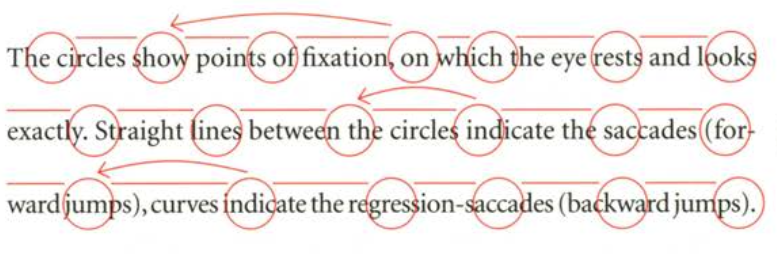
\includegraphics[scale=0.4]{img/saccade.png}
  \caption{The reading process.} 
  \label{fig:saccade}
\end{figure}

Therefore, keeping track of these saccades allows us to objectively access the legibility of a text. Not surprisingly, the same text will be read at differing speeds if systematic variations are made to the length of a line, the size/shape of the type, and the contrast between the color of the letters and their background. By acknowledging these rules, we can benefit in two ways. First, you can more accurately diagnose your own comprehension and speed when reading. Second, you can directly apply these rules to create ergonomic designs in your products. 
